\chapter{คู่มือการติดตั้งระบบ}
ในการติดตั้งเพื่อใช้งานแอปพลิเคชันระบบกองทุนเงินให้กู้ยืมเพื่อการศึกษา คณะวิทยาศาสตร์ มหาวิทยาลัยอุบลราชธานี หรือ ESP สามารถทำได้โดยมีขั้นตอนดังนี้
\begin{enumerate}
	\item สามารถดาวน์โหลด ESP installer package ได้ที่ https://drive.google.com/drive/folders/1k6HnoFgLAatgrfLAtFgnJYbRrpJHHwol ดังแสดงในรูปที่ \ref{Fig:dl1}
	\begin{figure}[H]
		\centering
		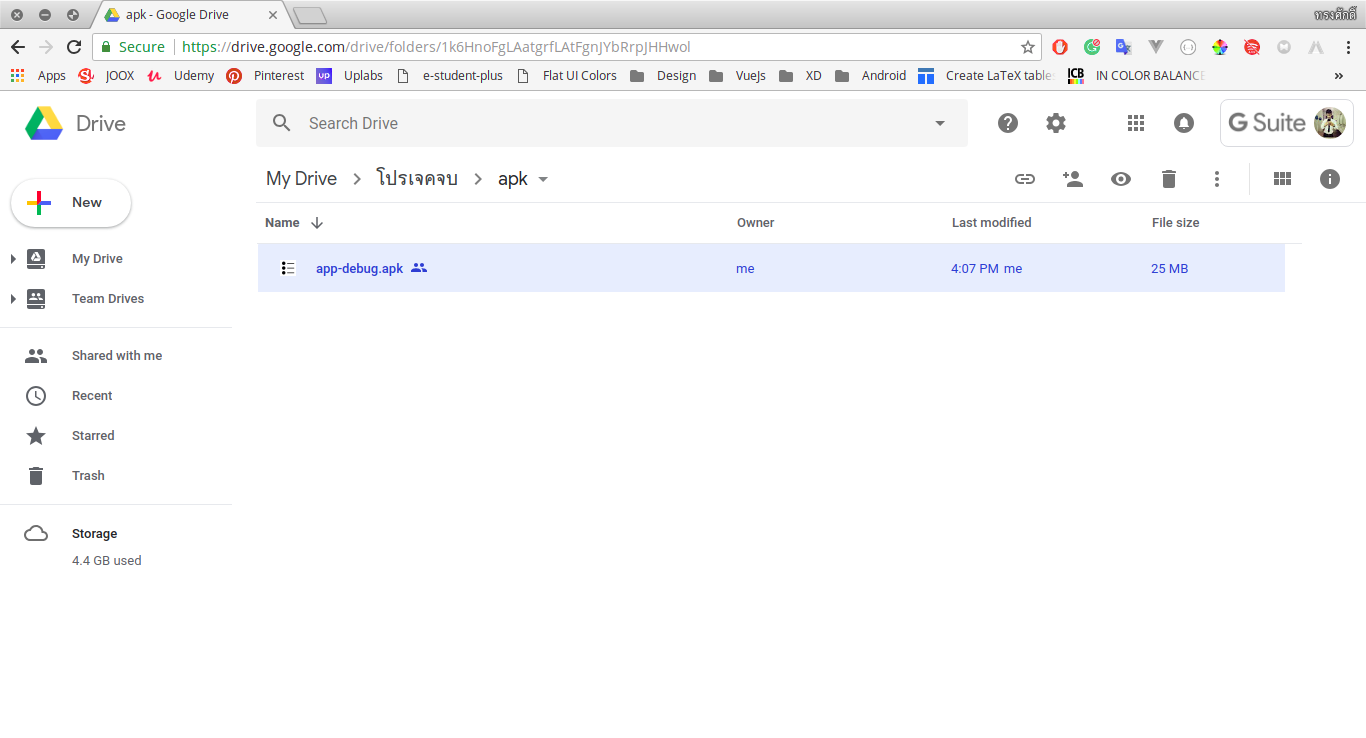
\includegraphics[width=\columnwidth]{Figures/7/installApp/dl}
		\caption{หน้าเว็บดาวน์โหลด ESP installer package}
		\label{Fig:dl1}
	\end{figure}
	\item ดัดลอกไฟล์ app-debug.apk ที่อยู่ในแฟ้มงาน(Folder)ที่อยู่บนคอมพิวเตอร์ไปไว้ในหน่วยความจำบนอุปกรณ์ที่ต้องการ ดังแสดงในรูปที่ \ref{Fig:dl2}
	\begin{figure}[H]
		\centering
		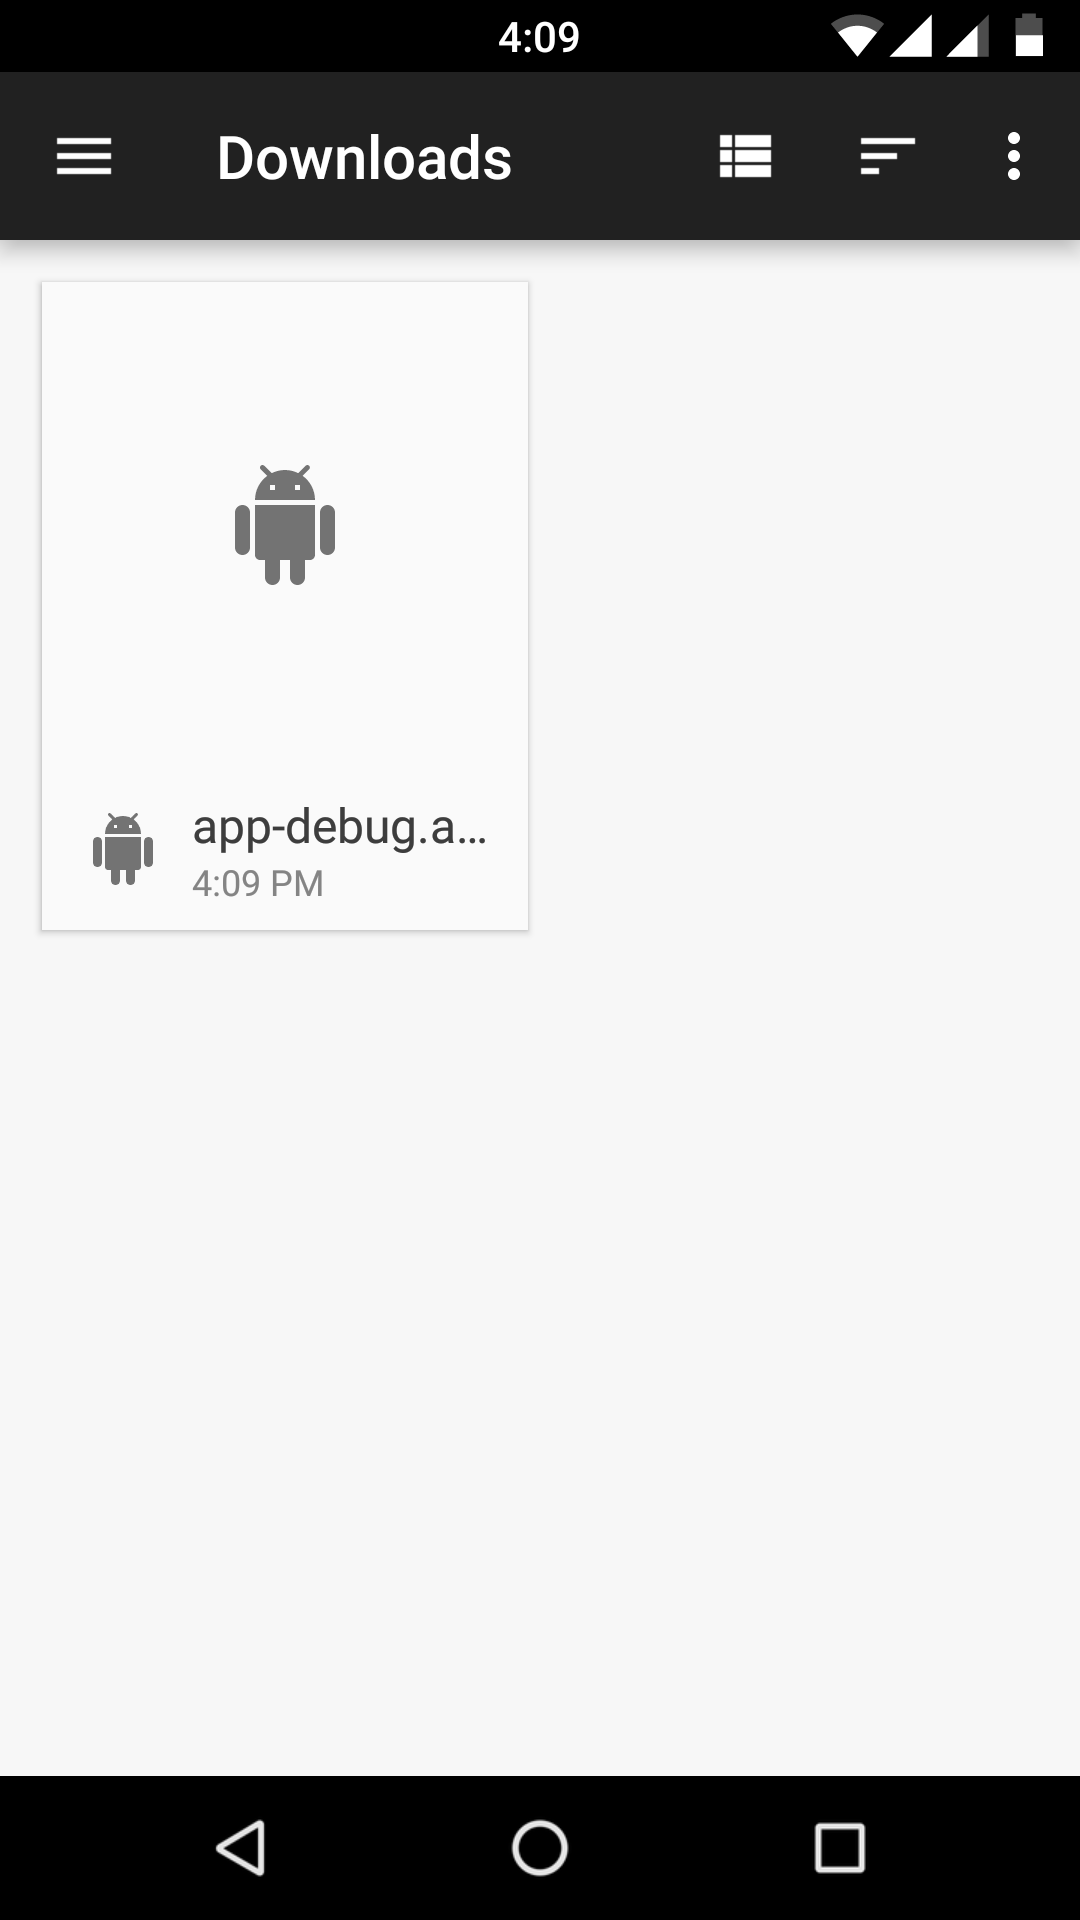
\includegraphics[width=0.3\columnwidth]{Figures/7/installApp/1}
		\caption{ไฟล์ app-debug.apk บนอุปรกรณ์}
		\label{Fig:dl2}
	\end{figure}
	\item  ทำการเปิดไฟล์ app-debug.apk และกด INSTALL เพื่อทำการติดตั้ง ดังแสดงในรูปที่ \ref{Fig:dl3}
	\begin{figure}[H]
		\centering
		
\includegraphics[width=0.3\columnwidth]{Figures/7/installApp/2}
		\caption{หน้าจอต้อนรับการติดตั้งแอปพลิเคชันบนอุปรกรณ์แอนดรอย์}
		\label{Fig:dl3}
	\end{figure}
	\item เมื่อทำการติดตั้งแอปพลิเคชันสำเร็จระบบจะแสดงผล ดังแสดงในรูปที่ \ref{Fig:dl4}
	\begin{figure}[H]
		\centering
		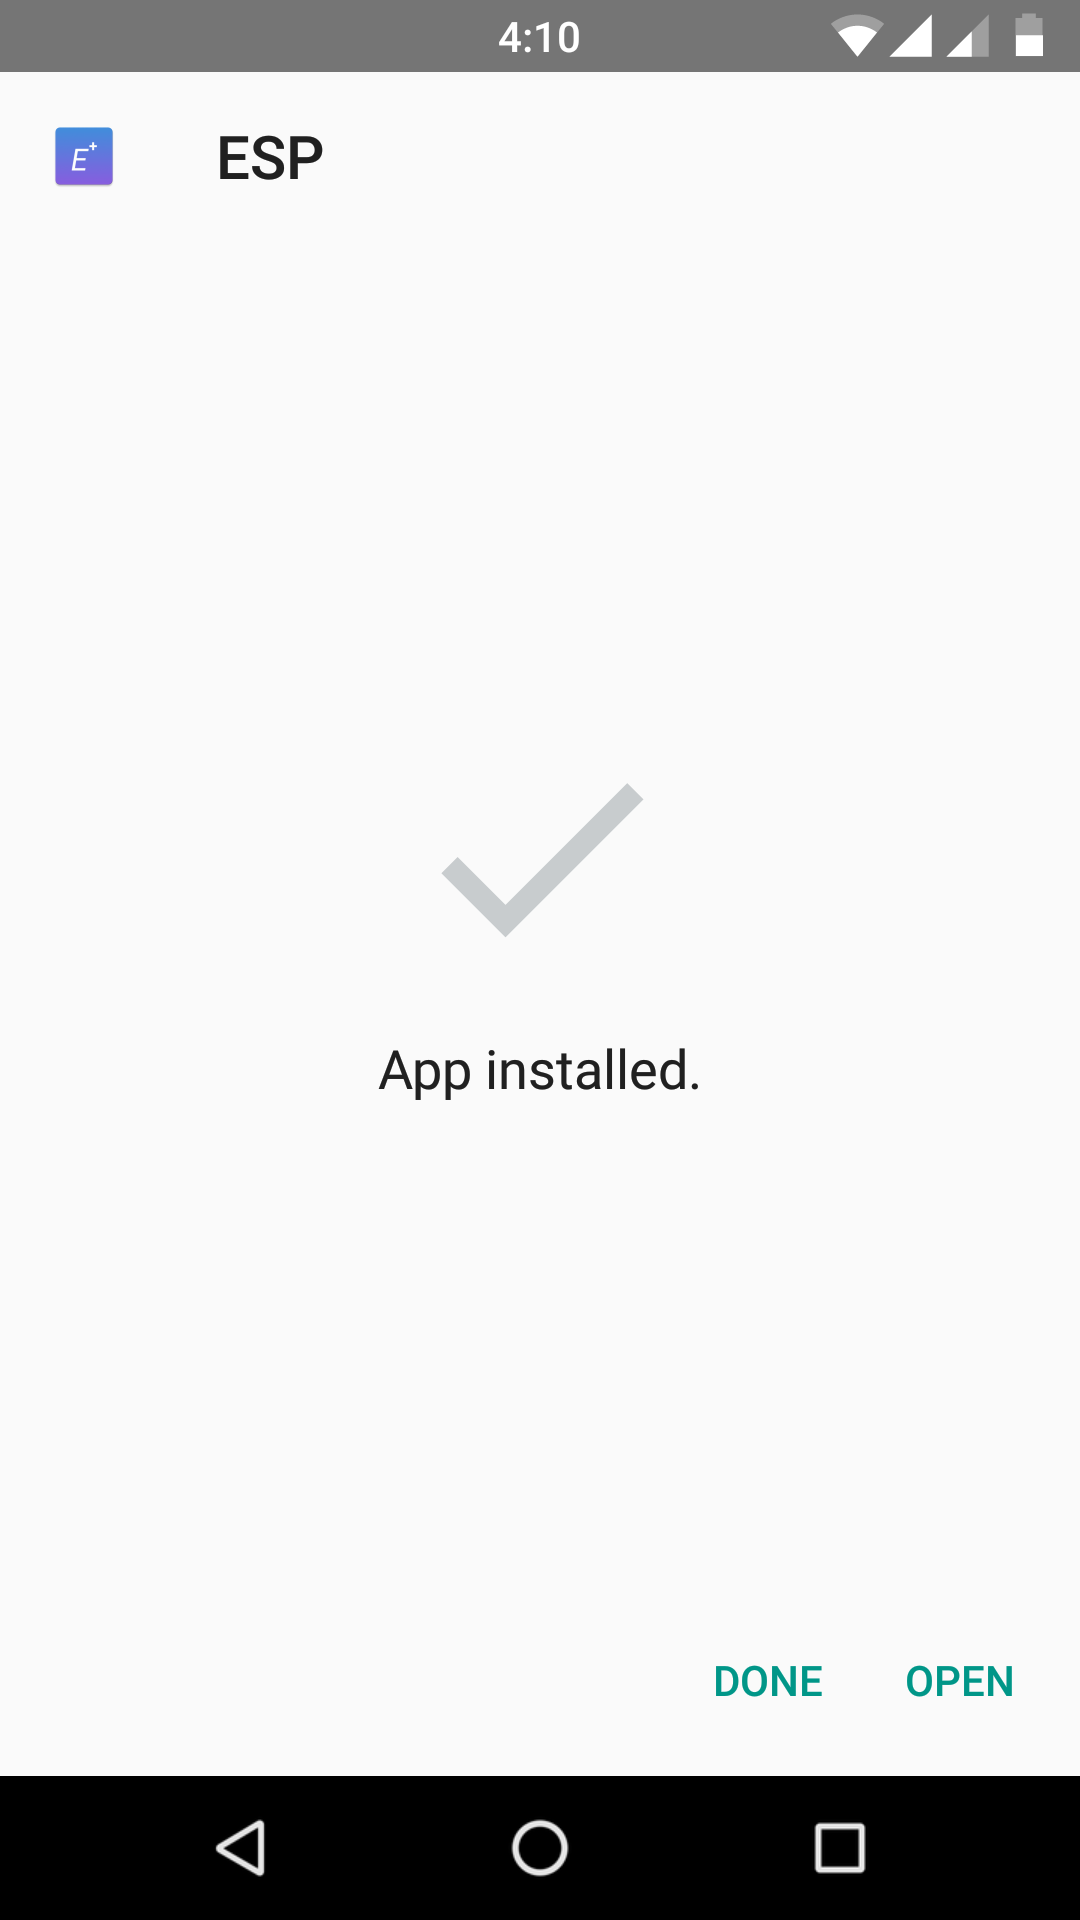
\includegraphics[width=0.3\columnwidth]{Figures/7/installApp/3}
		\caption{หน้าจอต้อนรับการติดตั้งแอปพลิเคชันบนอุปรกรณ์แอนดรอย์}
		\label{Fig:dl4}
	\end{figure}
\end{enumerate}
